\documentclass[numerate]{cheatsheet}
\usepackage{bm}
\usepackage{textcomp, mathcomp}
\usepackage{empheq}
\usepackage{pbox}
\usepackage{booktabs}

\lstset{style=python_style}

\doctitle{Informatik 2 Cheatsheet}
\author{Julian Lotzer – jlotzer@student.ethz.ch\\ 
Daniel Steinhauser – dsteinhauser@student.ethz.ch\\
Modified by:
Christian Leser - cleser@ethz.ch
\\ \vspace*{-0.2em}}

\begin{document}
\section{General Python}
	\subsection{Reference Semantics and Aliasing}
Everything is a pointer: l1 and l2 point to the same adress
\lstinputlisting{src/1_general_python/code/1_pointer_example.py}

If a copy is needed, use:
\lstinputlisting{src/1_general_python/code/1_copy_example.py}
    \subsection{Data Types}
    Python dynamically types variables, which means that the variable type can change during the program's execution
    \lstinputlisting{src/1_general_python/code/2_data_types.py}
    To convert the data type:
    \lstinputlisting{src/1_general_python/code/2_type_conversion.py}
    \subsubsection{Type Hints}
    help make code more legible
    \lstinputlisting{src/1_general_python/code/2_1_type_hints.py}
    \subsection{Input and Output}
    {\centering\underline{\textbf{Output}} \par}
    \lstinputlisting{src/1_general_python/code/3_output.py}
    {\centering\underline{\textbf{Input}} \par}
    \lstinputlisting{src/1_general_python/code/3_input.py}
    \subsection{Control Flows (if/else, while, for)}
    {\centering\underline{\textbf{if, else}} \par}
    \lstinputlisting{src/1_general_python/code/4_if_else.py}

    {\centering\underline{\textbf{while}} \par}
    \lstinputlisting{src/1_general_python/code/4_while.py}

    {\centering\underline{\textbf{for with range}} \par}
    \lstinputlisting{src/1_general_python/code/4_for_list.py}

    {\centering\underline{\textbf{for with lists}} \par}
    \lstinputlisting{src/1_general_python/code/4_for_range.py}

    \subsection{Functions}
    Functions do not have to be declared in a specific order
    \subsubsection{Function Declaration}
    \lstinputlisting{src/1_general_python/code/5_1_declaration.py}
    \subsubsection{Default arguments}
    When calling a function with default arguments, it is not necessary to call the function with arguments.
    \lstinputlisting{src/1_general_python/code/5_2_default_args.py}
    \subsubsection{Global and local variables}
    {\centering\textcolor{red}{Avoid this kind of code!} \par}
    global variables can be used within a function if declared before the funciton call. Also, local variables can be made global:
    \lstinputlisting{src/1_general_python/code/5_3_global_local.py}

\section{Python Containers}
    \subsection{Operations on Containers}
    Number of Elements:
\begin{lstlisting}
len(c)
\end{lstlisting}
    Contains element x?
\begin{lstlisting}
x in c
\end{lstlisting}
Iterate over all elements:
\begin{lstlisting}
for x in c:
print(x)
\end{lstlisting}
    \subsection{Sequences (ordered containers)}
    \subsubsection{Sequence Operations (Überarbeiten)} \label{section_sequence_operations}
Subscript-Operator l[i]:
\begin{lstlisting}
l = [1, 3, 'hi', -4]
print(l[2]) #output: hi
\end{lstlisting}
Enumeration:
\lstinputlisting{src/3_containers/code/2_1_enumeration.py}
Combine sequences s1 and s2 (zip):
\lstinputlisting{src/3_containers/code/2_1_zip.py}
Output with a for loop:
\lstinputlisting{src/3_containers/code/2_1_loop_output.py}
Slicing (partial sequence) of a sequence s:
\lstinputlisting{src/3_containers/code/2_1_slicing.py}
    \subsubsection{List (mutable)}
{\centering\underline{\textbf{Initialise a list with []}} \par}
\begin{lstlisting}
l = [1, 3, "hi", -4]
M = [[-1 for i in range(n)] for j in range(m)]
# 2D list or m x n-Matrix filled with -1
\end{lstlisting}

{\centering\underline{\textbf{Common List Operations}} \par}
\lstinputlisting{src/2_containers/code/2_2_list_operation.py}

{\centering\underline{\textbf{List Comprehension}} \par}
Apply a function $f(x)$ to all items in list l:
\begin{lstlisting}
l2 = [f(x) for x in l] #z.g. 2*x for f(x)
\end{lstlisting}
Apply a function $f(x)$ to a range:
\begin{lstlisting}
r2 = [f(x) for x in range(1,6)]
\end{lstlisting}
Apply a function $f(x)$ only to items in list l that satisfy $g(x)$ (filter):
\begin{lstlisting}
l3 = [f(x) for x in l if g(x)]
\end{lstlisting}
Example: Read a sequence of numbers:
\begin{lstlisting}
l = [int(x) for x in input("Input: ").split()]
\end{lstlisting}
    \subsubsection{Tuple (immutable)}
{\centering\underline{\textbf{Initialise a tuple}} \par}
\begin{lstlisting}
t = ("a", 0, -6, 3.3)
\end{lstlisting}
    \subsubsection{Range (immutable)}
{\centering\underline{\textbf{Initialise a range}} \par}
\begin{lstlisting}
#range(start, stop, step)
#befault: start = 0, step = 1, end not included
r = range(0, 8, 2) #r ->  0   2   4   6,
\end{lstlisting}
    \subsubsection{String (immutable)}
{\centering\underline{\textbf{Initialise a string}} \par}
\begin{lstlisting}
s = "hello" #s ->  'h' 'e' 'l' 'l' 'o'
#you can use both " or ' for strings 
\end{lstlisting}

{\centering\underline{\textbf{Common String Operations}} \par}
\lstinputlisting{src/2_containers/code/2_5_str_operations.py}
Example: check if s is a string with content:
\begin{lstlisting}
type(s) == str and len(s.strip()) #False if empty
\end{lstlisting}
To convert a string s to a list of words:
\begin{lstlisting}
s.split(seperator, maxsplit) 
#seperator and maxsplit are optional
#s.split() -> split at all whitespaces
#separator = ", " -> split at every ", "
#maxsplit = 10 -> split only at first 10 separators
\end{lstlisting}
    \subsection{Collections (unordered containers)}
    \subsubsection{Set (non-associative)}
{\centering\underline{\textbf{Initialise Set}} \par}
\begin{lstlisting}
s = {1, 29, 12}
\end{lstlisting}

{\centering\underline{\textbf{Common Set Operations}} \par}
\lstinputlisting{src/3_containers/code/3_1_set_operations.py}
    \subsubsection{Dictionary (associative)}
See \ref{section_sequence_operations} Sequence operations for 'enumerate' and 'zip'\\
{\centering\underline{\textbf{Initialise a Dictionary with \{\}}} \par}
A dictionary consists of \textbf{tuples (key, value)} as items. For that reason, one can think of it as a list of tuples (Which it is not in reality)
\lstinputlisting{src/3_containers/code/3_2_initialise_dict.py}

{\centering\underline{\textbf{Common Dictionary Operations}} \par}
\lstinputlisting{src/3_containers/code/3_2_dict_operations.py}

{\centering\underline{\textbf{Iterate over a Dictionary}} \par}
\lstinputlisting{src/3_containers/code/3_2_iterate_over_dict.py}

{\centering\underline{\textbf{Dictionary Comprehension}} \par}
Transform a set into a dictionary by applying $f(x)$ and $g(x)$ on every element in the set:
\begin{lstlisting}
d3 = {f(x):g(x) for x in s} #s being a set
d4 = {f(x):g(y) for x, y in z.items()} #z being a dict
\end{lstlisting}
Transform a set into a dictionary, only if the element satisfies h(x):
\begin{lstlisting}
d5 = {f(x):g(x) for x in s if h(x)}
\end{lstlisting}
Example: Multiply the value of every odd key in a dictionary by 2:
\begin{lstlisting}
d6 = {k:2*v for k, v in d.items() if k % 2 == 1}
\end{lstlisting}

\section{Numpy}
    Pandas is a Python package which supports working with tabulated data.

To import pandas, use:
\begin{lstlisting}
import pandas as pd
\end{lstlisting}

Now you can refer to classes and functions from the package using ”pd”.
    \subsection{Python Lists vs. Numpy Arrays}
Numpy arrays are like Python lists. Below is a summary of the key differences.
\begin{tabular*}{\linewidth}{m{0.44\linewidth} | m{0.44\linewidth}}
    Python Lists & Numpy Arrays\\
    \hline
    Variable size & Fixed size\\
    \hline
    Different element types & Single element type\\
    \hline
    Mathematical operations on single elements only & Mathematical operations on whole arrays\\
    \hline
    Primarily 1D & Multi-dimensional\\
\end{tabular*}

    \subsection{Declaring Numpy Arrays}
{\centering\underline{\textbf{Using sequences}} \par}
\lstinputlisting{src/3_numpy/code/3_sequence.py}

{\centering\underline{\textbf{Using random numbers}} \par}
\lstinputlisting{src/3_numpy/code/3_random.py}

{\centering\underline{\textbf{Using arange command}} \par}
creates an array from the start to the stop value with a given step value, stop is \textbf{not} inclusive
\lstinputlisting{src/3_numpy/code/3_arange.py}

{\centering\underline{\textbf{Using linspace command}} \par}
creates a numpy array with num equally spaced elements between start and stop, stop is inclusive:
\lstinputlisting{src/3_numpy/code/3_linspace.py}

\section{Pandas}

\section{Matplotlib}
    Pandas is a Python package which supports working with tabulated data.

To import pandas, use:
\begin{lstlisting}
import pandas as pd
\end{lstlisting}

Now you can refer to classes and functions from the package using ”pd”.
    \subsection{Line and Scatter Plots}
To graph two numpy arrays, one representing the x values and the other representing the corresponding y values:
\begin{minipage}{0.49\linewidth}
    \lstinputlisting{src/5_matplotlib/code/2_line_scatter.py}
\end{minipage}
\begin{minipage}{0.49\linewidth}
    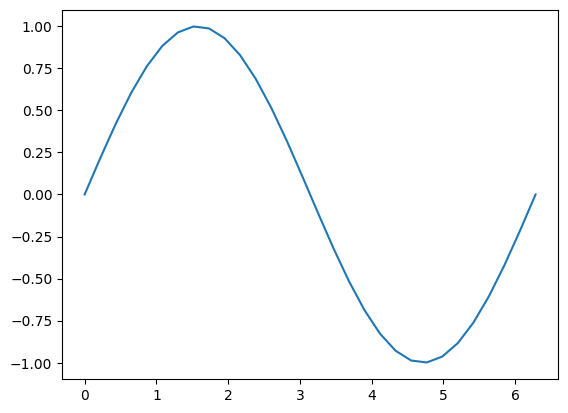
\includegraphics[width = \linewidth]{src/5_matplotlib/images/line_plot.png}
    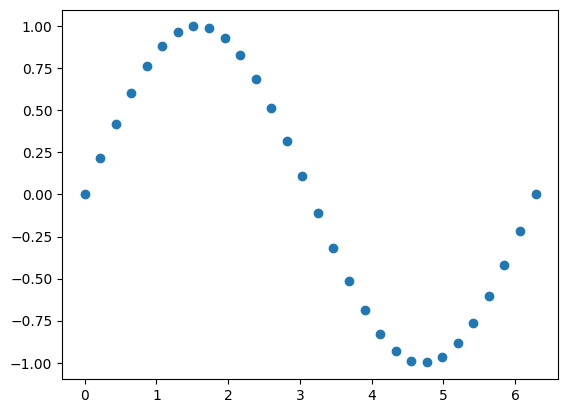
\includegraphics[width = \linewidth]{src/5_matplotlib/images/scatter_plot.png}
\end{minipage}

    \subsection{Histogram Plots}
To plot a histogram, use the following template:
\begin{minipage}{0.49\linewidth}
    \lstinputlisting{src/11_matplotlib/code/4_histogram.py}
\end{minipage}
\begin{minipage}{0.49\linewidth}
    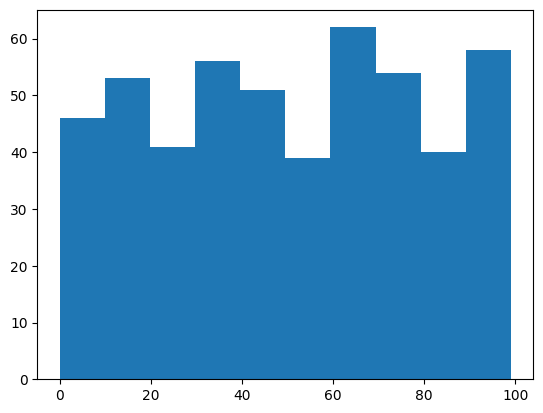
\includegraphics[width = \linewidth]{src/11_matplotlib/images/histogram_plot.png}
\end{minipage}


    \subsection{Graph Styling}
\lstinputlisting{src/5_matplotlib/code/5_styling.py}


\section{Algorithms}

\section{Data Structures}

\section{Programming Concepts}

\section{Dynamic Programming (DP)}

\section{Machine Learning (ML)}
\end{document}